% Figura cuerpo B2 (3.2.3): la objeción a CALVO: una probabilidad de reajuste que no mira al estado del precio
\documentclass[tikz,border=3pt]{standalone}
\usepackage[T1]{fontenc}
\usepackage[utf8]{inputenc}
\usepackage{amsmath}
\usetikzlibrary{arrows.meta,calc,positioning}
\begin{document}
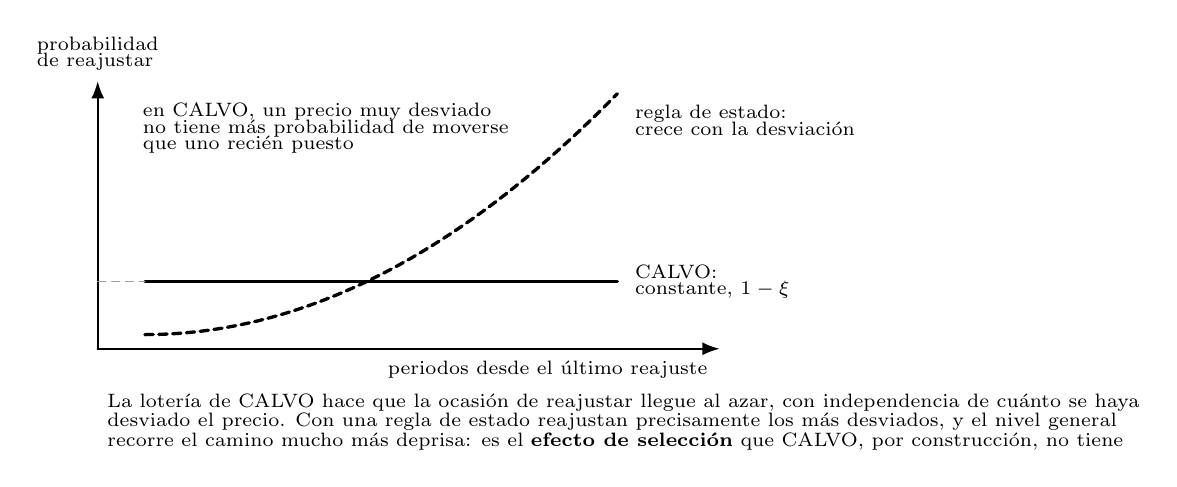
\begin{tikzpicture}[>={Latex[length=2.2mm]}, line cap=round, font=\footnotesize,
  eje/.style={->, thick},
  curva/.style={very thick},
  estado/.style={very thick, densely dashed},
  guia/.style={densely dashed, gray!75}]

  \draw[eje] (0,0) -- (7.9,0) node[below left=1pt, font=\scriptsize]{periodos desde el último reajuste};
  \draw[eje] (0,0) -- (0,3.4) node[above, font=\scriptsize, align=left]{probabilidad\\[-2pt]de reajustar};

  \draw[curva] (0.6,0.85) -- (6.6,0.85);
  \node[anchor=west, font=\scriptsize, align=left] at (6.7,0.85) {CALVO:\\[-2pt]constante, $1-\xi$};
  \draw[guia] (0,0.85) -- (0.6,0.85);

  \draw[estado] plot[domain=0.6:6.6, samples=60] ({\x},{0.18+0.085*(\x-0.6)*(\x-0.6)});
  \node[anchor=west, font=\scriptsize, align=left] at (6.7,2.90) {regla de estado:\\[-2pt]crece con la desviación};

  \node[anchor=west, font=\scriptsize, align=left] at (0.45,2.80)
    {en CALVO, un precio muy desviado\\[-2pt]no tiene más probabilidad de moverse\\[-2pt]que uno recién puesto};

  \node[align=left, anchor=north west, font=\scriptsize] at (0,-0.45)
    {La lotería de CALVO hace que la ocasión de reajustar llegue al azar, con independencia de cuánto se haya\\[-1pt]desviado el precio. Con una regla de estado reajustan precisamente los más desviados, y el nivel general\\[-1pt]recorre el camino mucho más deprisa: es el \textbf{efecto de selección} que CALVO, por construcción, no tiene};
\end{tikzpicture}
\end{document}
